\documentclass{article}
\usepackage[utf8]{inputenc}
\title{Lecture 10: Gradient Boosting}
\author{wbg231 }
\date{December 2022}
\newcommand{\R}{$\mathbb{R}$}
\newcommand{\B}{$\beta$}
\newcommand{\A}{$\alpha$}
\newcommand{\D}{\Delta}

\newcommand{\avector}[2]{(#1_2,\ldots,#1_{#2})}
\newcommand{\makedef}[2]{$\textbf{#1}$:#2 }
\usepackage{tikz,graphicx,hyperref,amsmath,amsfonts,amscd,amssymb,bm,cite,epsfig,epsf,url}

\begin{document}

\maketitle

\section*{introduction}
\begin{itemize}
\subsection*{today's lecture}
\item another way to get non-linear models in a linear form is with adaptive basis function models 
\item we are going to discuss a general greedy function approximation called gradient boosting machines 
\section{motivation}
\subsection{ada boost}
\item given training set $\mathcal{D}=\{(x_1,y_1)\cdots (x_n,y_n)\}$
\begin{enumerate}
    \item initialize observation weights $w_i=1$ for all i 
    \item for m=1 to M (number of trees we want to train) 
    \begin{itemize}
        \item base learner fits the training data and returns $G_M(x)$
        \item compute the weighted empirical 0-1 risk $$err_{m}=\frac{1}{W}w_i\mathbb{I}(y_i\neq G_m(x_i)) \text{   where } w=\Sigma_{i=1}^{n}w_i$$
        \item compute the classifier weight $\alpha_m=ln(\frac{1-err_m}{err_m}$
        \item update the example weight $w_i\leftarrow w_i \cdot e^{\alpha_m \mathbb{I}(y_i\neq G_m(x_i))}$
    \end{itemize}
    \item return final classifier $G(X)=sign[\Sigma_{m=1}^{m}\alpha_m G_m(x)]$
\end{enumerate}
\item why can we not just learn $G(x)$ directly? 
\item $G(X)$ is a linear sum of weak learners that could be non-linear and is learned sequentially 
\subsection{nonlinear regression}
\item how could we fit this data \\ 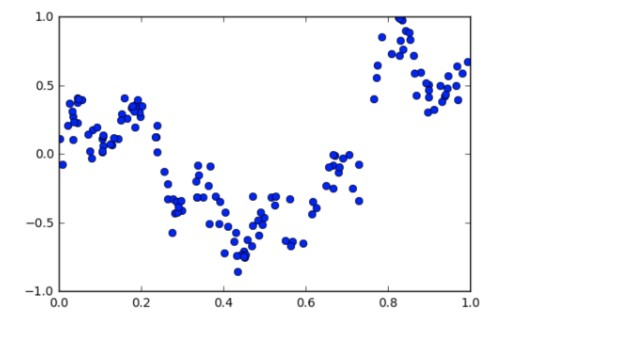
\includegraphics{lecture_notes/lecture_10/immages/l10_1.jpg}
\item using what we saw in ada boost we can fit a linear combination of transformations of the input that is $$f(x)=\Sigma_{m=1}^{M}v_{m}h_{m}(x)$$
 where $h_{i}(x)\forall i\in [1,m]$ are called the basis functions, (or feature functions) $$h_{i}:X\rightarrow \mathbb{R} \quad \forall i\in [1,M]$$
 \item an example could be polynomial regression where $h_{m}(x)=x^m$ and thus $f(x)=v_0+v_1x+v_2x^2+v_3x^3...+v_mx^m$ we have seen this before 
 \item can this model be expanded to classification tasks?
 \item yes we can fit this using standard methods for linear models (like least squares) 
 \item \textbf{note that our basis functions are picked ahead of time}
\subsection{adaptive basis model}
\item this type of model flips it so we want to learn (ie adapt) our basis function $h_{i}(x)$
\item call the base hypothesis space $\mathcal{H}=\{h:X\rightarrow \mathbb{R}\}$ that is the set of functions mapping from the input space to real numbers 
\item an \textbf{adaptive basis function expansion } over $\mathcal{H}$ is an ensemble model defined as $$f(x):=\Sigma_{m=1}^{M}v_{m}h_m(x)$$ where $v_m\in \mathbb{R} \text{ and } h_m\in \mathcal{H}$
\item thus we can call our combined hypothesis space $$F_{M}=\{\Sigma_{m=1}^{M}v_{m}h_m(x)|v_i\in \mathbb{R}, h_{i}\in \mathcal{H}, \forall i \in [1,m]\}$$
\item what are we learning in this? 
\subsection{empirical risk minimization }
\item recall the general learning objective is given by $$\hat{f}=argmin_{f\in \mathcal{F}_{n}}\frac{1}{n}\Sigma_{i=1}^{n}\ell(y_i,f(x_i))$$ for some loss function $\ell$
\item thus our erm objective for the adaptive basis function expansion is given as $$J(v_1,\cdots, v_m, h_1\cdots , h_m)=\frac{1}{n}\Sigma_{i=1}^{n}\ell(y_i,\Sigma_{m-1}^{M}v_mh_m(x))$$ 
\item the question  how do we optimize j is equivalent to asking how do we learn 
\subsection{gradient based methods}
\item let our base hypothesis space be parameterized by $\Theta=\mathbb{R}^{b}$
\item that is our basis functions $h_{i}(x)=\theta_i$
\item then we can write our objective as$$J(v_1,\cdots, v_m, \theta_1\cdots , \theta_m)=\frac{1}{n}\Sigma_{i=1}^{n}\ell(y_i,\Sigma_{m-1}^{M}v_m\theta_m(x))$$  
\item can we use SGD on this? 
\item it really depends on if our loss function $\ell$ and basis functions$\theta_{i}$ are differentiable 
\item so sometimes
\item neural nets are a differentiable case of this
\subsection{what if we can not do this}
\item what if the base hypothesis space $\mathcal{H}$ is decision trees
\begin{enumerate}
    \item we can not parameterize decision trees with $\Theta\in \mathbb{R}^{b}$ (our parameters are our splits)
    \item even if we could our predictions can not change continuously with respect to our parameters$\theta\in \Theta$ so they would not be differentiable 
\end{enumerate}
\item what about a greedy algorithm like ada boost?
\begin{enumerate}
    \item they work for both non parametric and non differentiable basis functions which is good
    \item does this count as optimizing our objective using some loss function?
\end{enumerate}
\item today we will discuss gradient boosting. 
\item this is more or less gradient descent in the feature space
\item it applies whenever we have 
\begin{enumerate}
    \item a loss function that is differentiable or sub differentiable with respect to the training predictions $f(x_i)$
    \item and we can do regression with the base hypothesis space $\mathcal{H}$
\end{enumerate}
\section{forward stagewise additive modeling }
\subsection{forward stagewise additive modeling  (FSAM)}
\item our goal is to fit a linear combination of basis functions $f(x)=\Sigma_{m=1}^{m}v_mh_m(x)$ given some loss function $\ell$
\item we do this by greedily fitting one function at a time while holding the previous functions constant. (that is at each stage we greedily pick the function $h_i(x)$ in our base hypothesis space that most reduces loss)
\item after $m-1$ stages we have $$f_{m-1}=\Sigma_{i=1}^{m-1}v_ih_i$$
\item in the mth round we want to find $h_m\in \mathcal{H}$ (ie a basis function) and weight $v_m\in \mathbb{R}>0$ such that $$f_m=f_{m-1}+v_mh_m$$ improves the objective as much as possible 
\item plugging this in we get 
\begin{enumerate}
    \item initialize $f_0(x)=0$
    \item for m=1 to M
    \begin{itemize}
        \item compute $$(v_m,h_m)=argmin_{v\in \mathbb{R}, h\in \mathcal{H}}\frac{1}{n}\Sigma_{i=1}^{n}\ell(y_i,f_{m-1}(x_i)+vh(x_i)$$
        \item then set $f_{m}=f_{m-1}+v_mh_m$
    \end{itemize}
    \item and return $f_M$
\end{enumerate}
\subsection{margin based classifiers}
\item the binary classification setup
\item outcome space $Y=\{-1,1\}$
\item the action space is $A=\mathbb{R}$ that is our model output
\item the score function $f:X\rightarrow A$
\item the margin for example i is $m=y_if(x_i)$ and $m>0\iff $ if our model prediction was correct. (and the larger M the better) 
\item the exponential loss function is given by $\ell_{exp}(y,f(x))=e^{-m}=e^{-yf(x)}$
\subsection{forward stagewise additive modeling function with exponential loss}
\item so our forward stagewise additive modeling function with exponential loss is given by 
\begin{enumerate}
    \item initialize $f_0(x)=0$
    \item for m=1 to M
    \begin{itemize}
        \item compute $$(v_m,h_m)=argmin_{v\in \mathbb{R}, h\in \mathcal{H}}\frac{1}{n}\Sigma_{i=1}^{n}\ell_{exp}(y_i,f_{m-1}(x_i)+vh(x_i)$$
        \item then set $f_{m}=f_{m-1}+v_mh_m$
    \end{itemize}
    \item and return $f_M$
\end{enumerate}
\item so the objective and the mth round is given by 
\item $j(v,h)=\Sigma_{i=1}^{n}e^{-y_i(x_{m-1}(x_i)+vh(x_i))}=\Sigma_{i=1}^{n}e^{-y_i(f_{m-1}(x_i)}e{-y_ivh(x_i))}=\Sigma_{i=1}^{n}w_{i}^{m}e{-y_ivh(x_i))}$
\item then we can expand this as $\Sigma_{i=1}^{N}w_{i}^{m}[\mathbb{I}(y_i=h(x_i))e^{-v}+\mathbb{I}(y_i\neq h(x_i))e^{v}]=\Sigma_{i=1}^{n}w_i^m[(e^{v}-e^{-v})\mathcal{I}(y_i\neq h(x_i) )+e^{-v}]$
\item given $v>0$ we have 
we have $\Sigma_{i=1}^{n}w_i^m[(e^{v}-e^{-v})\mathcal{I}(y_i\neq h(x_i) )+e^{-v}]=\Sigma_{i=1}^{n}w_i^m[(1)\mathcal{I}(y_i\neq h(x_i) )+e^{-v}]$
\item then given we only care about the section containing $h$
we have$armin_{h\in \mathcal{H}}j(v,h)=armin_{h\in \mathcal{H}}\Sigma_{i=1}^{n}w_{i}^{n}\mathbb{I}(y_i\neq h(x_i))=armin_{h\in \mathcal{H}}\Sigma_{i=1}^{n}\frac{1}{\Sigma_{i=1}^{n}w_i^{n}}w_{i}^{n}\mathbb{I}(y_i\neq h(x_i))=h_m$ since we are just multiplying by a constant in terms of h. 
\item so we can define weighted zero one error as $$err_{m}=\frac{\Sigma_{i=1}^{n}w_{i}^{m}\mathcal{I}(y_i\neq h(x_i)}{\Sigma_{i=1}^{n}w_i^m}$$ 
\item thus we can see that our $h_m$ are the functions in the basis space that minimize zero one loss
\item recall that our objective is given by $J(v,h)=\Sigma_{i=1}^{n}e^{-y_{i}(f_{m-1}(x_i)+vh(x_i))}=\Sigma_{i=1}^{n}e^{-y_if_{m-1}(x_i)}e^{-y_{i}vh(x_i)}=\Sigma_{i=1}^{n}w_{i}^{m}e^{-y_{i}vh(x_i)}$
\item so recall that the weight of individual i at iteration m is given by $w_{i}^{m}=e^{-y_if_{m-1}(x_i)}$
\item thus the weight of this next  round is $w_{i}^{m+1}=e^{-y_if_{m}(x_i)}=e^{-y_if_{m-1}(x_i)}e^{-y_iv_mh_m(x_i)}=w_{i}^{m}e^{-y_iv_mh_m(x_i)}=w_{i}^{m}e^{v_m\mathbb{I}(y_i\neq h_m(x_i)-v_m\mathbb{I}(y_i= h_m(x_i)}=w_i^{m}e^[wv_m\mathbb{I}(y_i\neq h_{m}(X_i))]e^{-v_m}$ where $e^{-v_m}$ is a scalar and thus will cancel out during normalization and can be safely ignored. 
\item so with exponential loss we find $f*(x)=\frac{1}{2}log\frac{p(y=1|x)}{P(y=0|x)}$ 
\item to do this derivation basically note that we are looking for the best loss given any x. so our goal is to minimize $\ell(y_i,f(x))=e^{-yf(x)}=e^{-f(x)+(1-y_i)f(x)}$ then just differentiate with respect to f(X)
\subsection{ada boost/ exponential loss robustness issues}
\item exponential loss by its nature puts  a lot of weight on miss classed examples which tends to lead to over fitting ie our model will not be robust to noise
\item ada boost does not do well with in stations with a lot of noise
\itme logistic loss preforms better in situations where there is a lot of randomness
\item exponential loss can have some computational advantages though 
\subsection{review}
\item so far we have seen 
\begin{enumerate}
    \item using a basis function to obtain nonlinear models $f(x)=\Sigma_{i=1}^{m}v_ih_i(x)$ with known basis functions $h_m(x)$
    \item adaptive models that do the same thing with unknown basis functions 
    \itme forward stagewise adaptive models that fit those basis to minimize average loss
\end{enumerate}
\item this however only works for certain loss functions we need a more general formula
\section{gradient boosting}
\subsection{consider fsam with squared loss}
\item if this is the case our objective at the mth round will be $$j(v,h)=\frac{1}{n}\Sigma_{i=1}^{n}\ell(y_i, f_m(x_i))=\frac{1}{n}\Sigma_{i=1}^{n}(y_i-f_{m-1}(x_i)-vh(x_i))^2$$
\item if our base hypothesis space $\mathcal{H}$ is closed under re scaling that is $\forall x\in \mathbb{R}, h\in \in \mathcal{H} xh\in \mathcal{H}$ then we don't need to learn v we can just learn h and v implicit.
\item so our problem becomes$$j(v,h)=\frac{1}{n}\Sigma_{i=1}^{n}\ell(y_i, f_m(x_i))=\frac{1}{n}\Sigma_{i=1}^{n}(y_i-f_{m-1}(x_i)-h(x_i))^2$$
\item note that $y_i-f_{m-1}(x_i)$ is the residual at step $m-1$, so this is fitting the residuals with least squares regression. that is we are more or less sequentially building models such that each marginal mode minimizes least squared of  the residual  
\subsection{example }
\item suppose we are fitting the following data using decision stumps that is models with only 1 condition 
\item 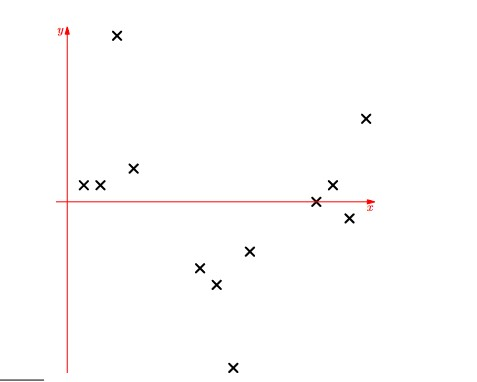
\includegraphics{lecture_notes/lecture_10/immages/l10_2.jpg}
\item here is what the stumps look like as time goes 
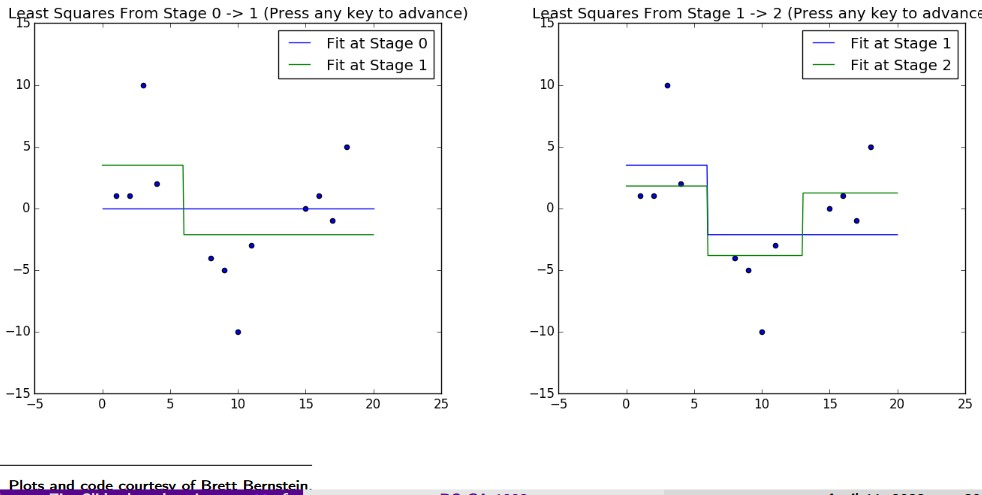
\includegraphics{lecture_notes/lecture_10/immages/l10_3.jpg}
\item 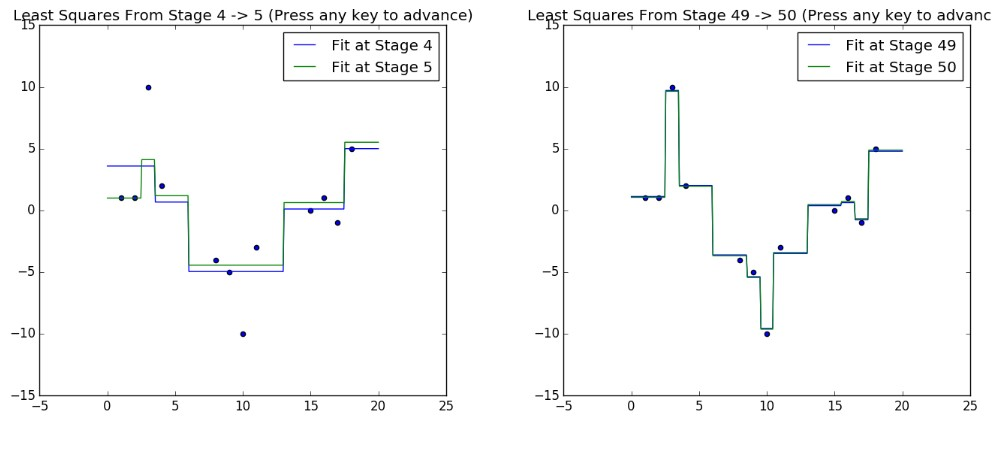
\includegraphics{lecture_notes/lecture_10/immages/l10_4.jpg}
\item so notice basically over time we can combine these models to fit a quite complex relationship
\subsection{interpret the residual}
\item once again note our objective is given by $$j(v,h)=\frac{1}{n}\Sigma_{i=1}^{n}\ell(y_i, f_m(x_i))=\frac{1}{n}\Sigma_{i=1}^{n}(y_i-f_{m-1}(x_i)-h(x_i))^2$$
\item so what is the residual at a specific data point $x_i$?
$j(v,h)=(y_i-f(x_i))^2$ thus $\nabla j_{f(x_i)}=-2(y_i-f(x_i))$
\item so our residual is the negative gradient 
\itme at each boosting round we can learn a function $h\in \mathcal{H}$ to fit the residual 
\item in boosting this is $f\leftarrow f+vh$
\item in gradient descent this is $f\leftarrow f-\alpha \nabla j(f)$
\item so h approximates the gradient and v approximates the negative step size
\subsection{functional gradient descent }
\item so our goal is to minimize $$j(f)=\Sigma_{i=1}^{n}\ell(y_i,f(x_i))$$
\item in some sense we want to take the gradient with respect to f 
\item j(f) only depends on g at n training points 
\item so we can define parameters of the form $\begin{pmatrix}
f(x_1)\\...\\f(x_n)
\end{pmatrix}$ that is the function evaluated at those points
\item the loss only really cares about the residual which is completely defined by the function evaluated at these n points
\item so we write our objective as $$j(f)=\Sigma_{i=1}^{n}\ell(y_i,f_i)$$
\item so think about the gradient of that objective 
\item the negative gradient step j is basically $g=-\nabla_{f}j(f)=-\begin{pmatrix}
\partial \ell(y_1,f_1)    
\end{pmatrix}$ that is the gradient is the vector of partial derivatives of the loss of the each training point given the function f. which can be calculated
\item $-g\in \mathbb{R}^{n}$ is the direction we want to change each of our n predictions towards for all points in the training data. 
\item in gradient descent  our final predictor will be $f_{0}+\Sigma_{m=1}^{M}v_T(-g_t)$ so effectively a very carefully reweighing or initial model 
\item we call these $g=-\nabla_{f}j(f)=-\begin{pmatrix}
\partial \ell(y_1,f_1)    
\end{pmatrix}$
the pseudo residuals (for square loss they are just the residuals)
\item our pseudo-residuals are the unconstrained step direction (ie if we could adjust our function however we wanted that is how we would do so)
\item the problem is we only know how to update at n points, how do we take a gradient step in $\mathcal{H}$
\item we approximate the closest base mode $h\in \mathcal{H}$ that is $$min_{h\in \mathcal{H}}\Sigma_{i=1}^{N}(-g_{i}-h(x_i))^2$$ (here we are assumption that we are using l2 distance but that does not necessarily have to be the case 
\item so we take the $h\in \mathcal{H}$ that best approximates our step direction
\subsection{functional gradient descent hyper parameters}
\item we chose a step size with line search $$v_{m}=argmin_{v}\Sigma_{i=1}^{n}\ell(y_i, f_{m-1}(x_i)+vh_m(x_i))$$ ie we adjust v as we go and take the v that minimizes loss
\item we also add regularization with a shrinkage parameter $\lamnda \in [0,1]$ such that $$f_{m}\leftarrow f_{m-1}+\lambda v_{m}h_m$$
\item then we chose the number of iterations we do based on the validation set 
\subsection{gradient boost algorithm}
\item initialize f to a constant $f_{0}=armin_{\gamma \in \mathbb{R}}\ell(y_i, \gamma)$
\item for m from 1 to M
\begin{enumerate}
    \item compute the pseudo-residuals (negative gradient) $$r_{im}=[\frac{\partial \ell(y_i,f(x_i))}{\partial f(x_i)}]$$ where $f(x_i)=f_{m-1}(x_i)$
    \item optional find the best step size $v_{m}=argmin_{v}\Sigma_{i=1}^{n}\ell(y_i, f_{m-1}(x_i)+vh_m(x_i))$
    \item update $f_m=f_{m-1}+\lambda v_m h_m$
\end{enumerate}
\item return $f_M(x)$
\subsection{gradient boosting machine ingredients }
\item take any loss function (that is sub differentiable) with respect to it''s predictions $f(x_i)$ 
\item chose  abase hypothesis space for regression $\mathcal{H}$
\item chose a number of steps $M$
\item chose a step size methodology (that is how you set that hyper parameter) 
\subsection{binomial boost}
\item gradient boost with logistic loss is called binomial boost
\item we are working with an input space $y\in \{-1,1\}$
\item and loss function $$\ell(y,f(x))=log(1+e^{-yf(x)}$$
\item we can see that the pseudo residual  of the ith example with respect to it's prediction is 
$r_i=-\frac{\partail \ell(y_i,f(x))}{\partial f(x_i)}=-\frac{\partial}{\partial f(x_i)}log(1+e^{-y_{i}f(x_i)}=\frac{y_ie^{-y_if(x_i)}}{1+e^{-y_if(x_i)}}=\frac{y_ie^{-y_if(x_i)}}{1+e^{-y_if(x_i)}}*\frac{e^{y_if(x_i)}}{e^{y_if(x_i)}}=\frac{y_i}{1+e^{y_if(x_i)}}$
\item so if $f_{m-1}(x)$ is the prediction after m-1 rounds, the step direction at the mth round is $$h_{m}=armin_{h\in \mathcal{H}}\Sigma_{i=1}^{n}(\frac{y_i}{1+e^{y_if_{m-1}(x_i)}}-h(x_i))^2$$
\item and $f_{m}(x)=f_{m-1}(x)+vh_{m}(x)$
\subsection{gradient tree boosting }
\item one common from of gradient boosting machine takes $$\mathcal{H}=\{\text{regression tree of size S}\}$$
that is each of our base estimators are regression trees with S terminal nodes.
\item s=2 gives decision stumps (ie 2 splits) 
\item recent studies use larger trees
\item there are a lot of packages that incorporate this. 
\item this works really well in practice
\section{in practice}
\subsection{prevent over fitting}
\item boosting is resilient to over fitting for the following reasons 
\begin{enumerate}
    \item there is implicit feature selection we are greedily selecting the best feature at each step 
    \item and as the training goes on the in pact of training is localized to a few data points 
\end{enumerate}
\itme but it can overfit so we can try to regularize with 
\begin{itemize}
    \item shrinkage (small learning rate)
    \item stochastic gradient boosting (taking subsections of rows)
    \item feature sub sampling (that is taking subsections of features)
\end{itemize}
\item set step size as small as you can/have the patience for it can only prevent over fitting more
\subsection{stochastic gradient boosting }
\item at each state we chose a random sub sample of the data for computing projected gradient step 
\item this is good because we introduce randomness to prevent over fitting  and it is faster 
\itme this is pretty much mini batch stochastic gradient descent 
\subsection{feature sub sampling}
\item this is kind of similar to random forests, we random chose a subset of features for each round to learn from 
\item it also lowers complexity so makes computation faster

\subsection{summary}
\item the idea of boosting is to combine weak learners to produce a strong learner 
\item from the statistical perspective boosting is fitting an additive model (greedily) 
\itme from the numerical optimization perspective boosting makes local improvements iterative that is gradient descent in the feature space. 
\item gradient boosting is a generic framework so can be applied all over. 


\end{itemize}
\end{document}
